% ===========================================================
%  COMP0497 — Algoritmos e Estruturas de Dados I
%  Ordenação: Merge Sort, Quick Sort, Limites e Counting Sort
%  Prof. Dr. André Yoshiaki Kashiwabara — DCOMP/UFS
% ===========================================================
\documentclass[aspectratio=169]{beamer}

\usepackage[T1]{fontenc}
\usepackage[utf8]{inputenc}
\usepackage{xcolor}

% ---- Cores customizadas -------------------------------------
\definecolor{UFSBlue}{RGB}{0,84,166}
\definecolor{sicpGreen}{RGB}{0,140,70}
\definecolor{alertRed}{RGB}{180,30,30}
\definecolor{arrayFill}{RGB}{220,235,255}
\definecolor{arrayHL}{RGB}{255,220,100}
\definecolor{mergeHL}{RGB}{200,255,200}
\definecolor{pivotColor}{RGB}{255,180,180}
\definecolor{ltColor}{RGB}{200,240,200}
\definecolor{gtColor}{RGB}{240,210,180}

% ---- Tema UFS -----------------------------------------------
\usetheme{UFS}
\usecolortheme[named=UFSBlue]{structure}
\setbeamertemplate{navigation symbols}{}
\setbeamertemplate{footline}[frame number]

% ---- Pacotes ------------------------------------------------
\usepackage{amsmath,amssymb,amsthm}
\usepackage{tikz}
\usetikzlibrary{arrows,shapes,positioning,calc,decorations.pathreplacing,fit}
\usepackage{algorithm}
\usepackage{algpseudocode}
\usepackage{listings}

\lstset{
  basicstyle=\ttfamily\small,
  numbers=left,
  numberstyle=\tiny\color{gray},
  stepnumber=1,
  numbersep=5pt,
  frame=single,
  breaklines=true,
  tabsize=2,
  morekeywords={for,to,downto,return,if,then,else,end,do,while},
  keywordstyle=\bfseries,
  commentstyle=\itshape\color{gray!70},
  morecomment=[l]{//}
}

% ---- Comando inline Python/código ---------------------------
\newcommand{\py}[1]{\texttt{\color{UFSBlue}#1}}

% ---- Estilos TikZ -------------------------------------------
\tikzstyle{cellbox}=[draw, minimum width=0.65cm, minimum height=0.65cm, fill=arrayFill, font=\small]
\tikzstyle{cellhl}=[draw, minimum width=0.65cm, minimum height=0.65cm, fill=arrayHL, font=\small\bfseries]
\tikzstyle{cellmerge}=[draw, minimum width=0.65cm, minimum height=0.65cm, fill=mergeHL, font=\small\bfseries]
\tikzstyle{treenode}=[circle, draw=UFSBlue, fill=arrayFill, minimum size=0.7cm, font=\small]
\tikzstyle{treeleaf}=[rectangle, draw=sicpGreen!70!black, fill=sicpGreen!15, minimum width=1.1cm, minimum height=0.55cm, font=\scriptsize, rounded corners=2pt]
\tikzstyle{treearrow}=[->, >=stealth', thick, color=gray!70]
\tikzstyle{rectnode}=[rectangle, draw=UFSBlue, fill=arrayFill, rounded corners=2pt, minimum width=1.6cm, minimum height=0.6cm, font=\small]
\tikzstyle{splitarrow}=[->, >=stealth', thick, color=UFSBlue]
\tikzstyle{mergearrowstyle}=[->, >=stealth', thick, color=sicpGreen!80!black]

% Estilos QuickSort
\tikzstyle{cell}=[draw, minimum width=0.68cm, minimum height=0.68cm, fill=arrayFill, font=\small]
\tikzstyle{cellpivot}=[draw, minimum width=0.68cm, minimum height=0.68cm, fill=pivotColor, font=\small\bfseries]
\tikzstyle{celllt}=[draw, minimum width=0.68cm, minimum height=0.68cm, fill=ltColor, font=\small]
\tikzstyle{cellgt}=[draw, minimum width=0.68cm, minimum height=0.68cm, fill=gtColor, font=\small]
\tikzstyle{celldone}=[draw, minimum width=0.68cm, minimum height=0.68cm, fill=sicpGreen!25, font=\small]
\tikzstyle{worstarrow}=[->, >=stealth', thick, color=alertRed]
\tikzstyle{avgbox}=[rectangle, draw=sicpGreen!80!black, fill=sicpGreen!12, rounded corners=3pt, minimum width=3.6cm, minimum height=0.7cm, font=\small]

% Estilos Limite Inferior
\tikzstyle{decnode}=[ellipse, draw, fill=blue!15, minimum width=2.2cm, minimum height=0.7cm, font=\small]
\tikzstyle{leafnode}=[rectangle, draw, fill=green!20, rounded corners, minimum width=1.2cm, minimum height=0.6cm, font=\scriptsize]
\tikzstyle{treeedge}=[->, >=stealth', thick]
\tikzstyle{thinedge}=[->, >=stealth', thin]

% Estilos Counting Sort
\tikzstyle{cellh}=[rectangle, draw=blue!70, fill=blue!20, minimum width=0.7cm, minimum height=0.7cm, font=\small\bfseries, inner sep=2pt]
\tikzstyle{cellout}=[rectangle, draw=green!60!black, fill=green!15, minimum width=0.7cm, minimum height=0.7cm, font=\small\bfseries, inner sep=2pt]
\tikzstyle{myarrow}=[->, >=stealth', thick]

% ---- Metadados ----------------------------------------------
\title{Merge Sort, Quick Sort, Limite Inferior e Counting Sort}
\author{Prof.\ Dr.\ André Yoshiaki Kashiwabara}
\institute{DCOMP --- Universidade Federal de Sergipe}
\date{}
% =============================================================
\begin{document}

\begin{frame}
  \titlepage
\end{frame}

% =============================================================
% MERGE SORT
% =============================================================
\part{Merge Sort}
\section{Merge Sort}

\begin{frame}{Merge Sort: Motivação}
  \begin{columns}[T]
    \begin{column}{0.54\textwidth}
      \begin{itemize}
        \item Insertion Sort: $\Theta(n^2)$ no pior caso\\[4pt]
        \item Podemos fazer melhor?
          \begin{itemize}
            \item \textbf{Sim!} Usando \emph{divisão e conquista}
          \end{itemize}
        \item \textbf{Merge Sort}: $\Theta(n \log n)$ em \emph{todos} os casos
        \item Algoritmo \emph{estável} e \emph{paralelizável}
        \item Base para variantes externas (External Merge Sort)
      \end{itemize}
    \end{column}
    \begin{column}{0.42\textwidth}
      \begin{center}
        \renewcommand{\arraystretch}{1.3}
        \begin{tabular}{lc}
          \hline
          \textbf{Algoritmo} & \textbf{Pior caso} \\
          \hline
          Insertion Sort & $\Theta(n^2)$ \\
          Merge Sort     & $\Theta(n \log n)$ \\
          Quick Sort     & $\Theta(n^2)$ \\
          \hline
        \end{tabular}
      \end{center}
    \end{column}
  \end{columns}
\end{frame}

\begin{frame}{Paradigma Divisão e Conquista}
  \begin{block}{Três etapas}
    \begin{enumerate}
      \item \textbf{Dividir}: quebrar o problema em subproblemas menores
      \item \textbf{Conquistar}: resolver recursivamente (ou diretamente se trivial)
      \item \textbf{Combinar}: juntar as soluções parciais
    \end{enumerate}
  \end{block}

  \vspace{6pt}
  \begin{exampleblock}{No Merge Sort}
    \begin{itemize}
      \item \textbf{Dividir}: partir $A[p \ldots r]$ ao meio em $A[p \ldots q]$ e $A[q{+}1 \ldots r]$
      \item \textbf{Conquistar}: ordenar recursivamente cada metade
      \item \textbf{Combinar}: intercalar (\emph{merge}) as duas metades ordenadas
    \end{itemize}
  \end{exampleblock}
\end{frame}

\begin{frame}[fragile]{Merge Sort — pseudocódigo}
  \begin{algorithm}[H]
    \caption{\textsc{MergeSort}$(A, p, r)$}
    \begin{algorithmic}[1]
      \If{$p < r$}
        \State $q \gets \lfloor (p + r) / 2 \rfloor$
        \State \textsc{MergeSort}$(A, p, q)$
        \State \textsc{MergeSort}$(A, q{+}1, r)$
        \State \textsc{Merge}$(A, p, q, r)$
      \EndIf
    \end{algorithmic}
  \end{algorithm}

  \vspace{8pt}
  \begin{itemize}
    \item Chamada inicial: \textsc{MergeSort}$(A, 1, n)$
    \item Caso base: subarray de tamanho $\leq 1$ já está ordenado
    \item O \emph{trabalho real} acontece na etapa \textbf{Combine}: \textsc{Merge}
  \end{itemize}
\end{frame}

\begin{frame}[fragile,shrink=5]{Procedimento \textsc{Merge}}
  \begin{algorithm}[H]
    \caption{\textsc{Merge}$(A, p, q, r)$}
    \begin{algorithmic}[1]
      \State Copiar $A[p..q]$ para $L[1..|L|]$ e $A[q{+}1..r]$ para $R[1..|R|]$
      \State Adicionar sentinela $\infty$ ao final de $L$ e $R$
      \State $i \gets 1$; \; $j \gets 1$
      \For{$k \gets p$ \textbf{to} $r$}
        \If{$L[i] \leq R[j]$}
          \State $A[k] \gets L[i]$; \; $i \gets i + 1$
        \Else
          \State $A[k] \gets R[j]$; \; $j \gets j + 1$
        \EndIf
      \EndFor
    \end{algorithmic}
  \end{algorithm}

  \vspace{4pt}
  \begin{itemize}
    \item Complexidade de \textsc{Merge}: $\Theta(n)$ — percorre $r - p + 1$ posições
    \item Sentinela $\infty$ simplifica o código (evita checar fim de lista)
  \end{itemize}
\end{frame}

\begin{frame}{Visualização: divisão recursiva}
  \centering
  \resizebox{0.95\textwidth}{!}{%
  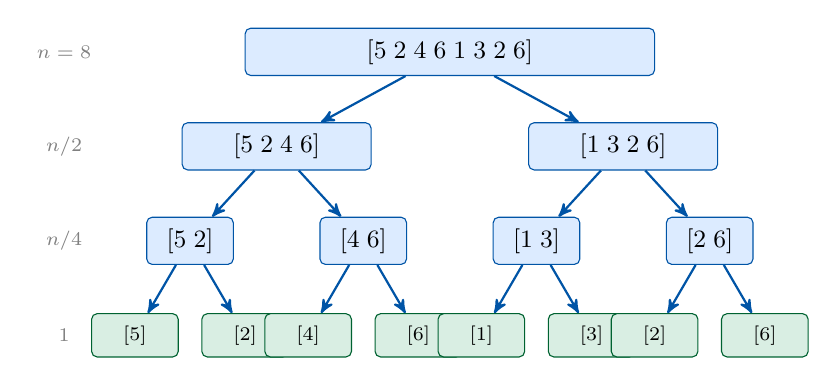
\begin{tikzpicture}[node distance=0.5cm and 0.2cm]
    % Nível 0
    \node[rectnode, minimum width=5.2cm] (n0) at (4,4)
      {$[5\;2\;4\;6\;1\;3\;2\;6]$};

    % Nível 1
    \node[rectnode, minimum width=2.4cm] (n1l) at (1.8,2.8)
      {$[5\;2\;4\;6]$};
    \node[rectnode, minimum width=2.4cm] (n1r) at (6.2,2.8)
      {$[1\;3\;2\;6]$};

    % Nível 2
    \node[rectnode, minimum width=1.1cm] (n2a) at (0.7,1.6)  {$[5\;2]$};
    \node[rectnode, minimum width=1.1cm] (n2b) at (2.9,1.6)  {$[4\;6]$};
    \node[rectnode, minimum width=1.1cm] (n2c) at (5.1,1.6)  {$[1\;3]$};
    \node[rectnode, minimum width=1.1cm] (n2d) at (7.3,1.6)  {$[2\;6]$};

    % Nível 3 (folhas)
    \node[treeleaf] (l1) at (0,0.4)   {$[5]$};
    \node[treeleaf] (l2) at (1.4,0.4) {$[2]$};
    \node[treeleaf] (l3) at (2.2,0.4) {$[4]$};
    \node[treeleaf] (l4) at (3.6,0.4) {$[6]$};
    \node[treeleaf] (l5) at (4.4,0.4) {$[1]$};
    \node[treeleaf] (l6) at (5.8,0.4) {$[3]$};
    \node[treeleaf] (l7) at (6.6,0.4) {$[2]$};
    \node[treeleaf] (l8) at (8.0,0.4) {$[6]$};

    % Setas de divisão
    \draw[splitarrow] (n0) -- (n1l);
    \draw[splitarrow] (n0) -- (n1r);
    \draw[splitarrow] (n1l) -- (n2a);
    \draw[splitarrow] (n1l) -- (n2b);
    \draw[splitarrow] (n1r) -- (n2c);
    \draw[splitarrow] (n1r) -- (n2d);
    \draw[splitarrow] (n2a) -- (l1);
    \draw[splitarrow] (n2a) -- (l2);
    \draw[splitarrow] (n2b) -- (l3);
    \draw[splitarrow] (n2b) -- (l4);
    \draw[splitarrow] (n2c) -- (l5);
    \draw[splitarrow] (n2c) -- (l6);
    \draw[splitarrow] (n2d) -- (l7);
    \draw[splitarrow] (n2d) -- (l8);

    % Rótulo de níveis
    \node[font=\scriptsize\color{gray}] at (-0.9,4)   {$n=8$};
    \node[font=\scriptsize\color{gray}] at (-0.9,2.8) {$n/2$};
    \node[font=\scriptsize\color{gray}] at (-0.9,1.6) {$n/4$};
    \node[font=\scriptsize\color{gray}] at (-0.9,0.4) {$1$};
  \end{tikzpicture}}%
\end{frame}

\begin{frame}{Visualização: passo de \textsc{Merge}}
  \centering
  \vspace{4pt}
  {\small Intercalando $L = [2,5]$ e $R = [1,4]$ em $A$:}

  \vspace{8pt}
  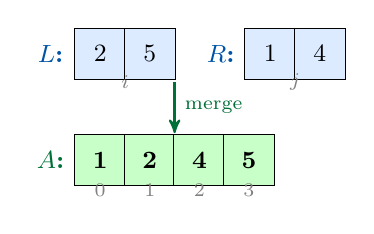
\begin{tikzpicture}[scale=0.9]
    % Arrays L e R
    \foreach \val/\i in {2/0,5/1} {
      \node[cellbox] at (\i*0.7, 1.5) {\val};
    }
    \node[font=\small\bfseries, color=UFSBlue] at (-0.7, 1.5) {$L$:};
    \node[font=\scriptsize, color=gray] at (0.35, 1.1) {$i$};

    \foreach \val/\i in {1/0,4/1} {
      \node[cellbox] at (2.4+\i*0.7, 1.5) {\val};
    }
    \node[font=\small\bfseries, color=UFSBlue] at (1.7, 1.5) {$R$:};
    \node[font=\scriptsize, color=gray] at (2.75, 1.1) {$j$};

    % Array resultado (4 passos)
    \node[font=\small\bfseries, color=sicpGreen!80!black] at (-0.7, 0) {$A$:};
    \node[cellmerge]  at (0.0,  0) {1};
    \node[cellmerge]  at (0.7,  0) {2};
    \node[cellmerge]  at (1.4,  0) {4};
    \node[cellmerge]  at (2.1,  0) {5};
    \foreach \i in {0,...,3} {
      \node[font=\scriptsize, color=gray] at (\i*0.7, -0.42) {\i};
    }

    % Seta indicando sentido da construção
    \draw[mergearrowstyle] (1.05, 1.1) -- (1.05, 0.38)
          node[midway, right, font=\scriptsize] {merge};
  \end{tikzpicture}

  \vspace{8pt}
  \begin{itemize}
    \item A cada passo: comparar $L[i]$ e $R[j]$, copiar o menor para $A$
    \item Total: $r - p + 1$ comparações/cópias $\Rightarrow$ $\Theta(n)$
  \end{itemize}
\end{frame}

\begin{frame}{Recorrência do Merge Sort}
  \begin{block}{Equação de recorrência}
    \[
      T(n) = \begin{cases}
        \Theta(1) & \text{se } n = 1 \\
        2\,T\!\left(\dfrac{n}{2}\right) + \Theta(n) & \text{se } n > 1
      \end{cases}
    \]
  \end{block}

  \vspace{8pt}
  \begin{columns}[T]
    \begin{column}{0.48\textwidth}
      \textbf{Interpretação:}
      \begin{itemize}
        \item $2T(n/2)$: duas chamadas recursivas de tamanho $n/2$
        \item $\Theta(n)$: custo do \textsc{Merge}
      \end{itemize}
    \end{column}
    \begin{column}{0.48\textwidth}
      \textbf{Solução:}
      \[
        T(n) = \Theta(n \log n)
      \]
      \begin{itemize}
        \item Pelo \emph{Teorema Mestre} (caso 2):\\
              $a=2,\; b=2,\; f(n)=\Theta(n)$\\
              $n^{\log_b a} = n^1 \Rightarrow$ caso 2
      \end{itemize}
    \end{column}
  \end{columns}
\end{frame}

\begin{frame}[shrink=5]{Análise pela Árvore de Recursão}
  \centering
  \resizebox{0.97\textwidth}{!}{%
  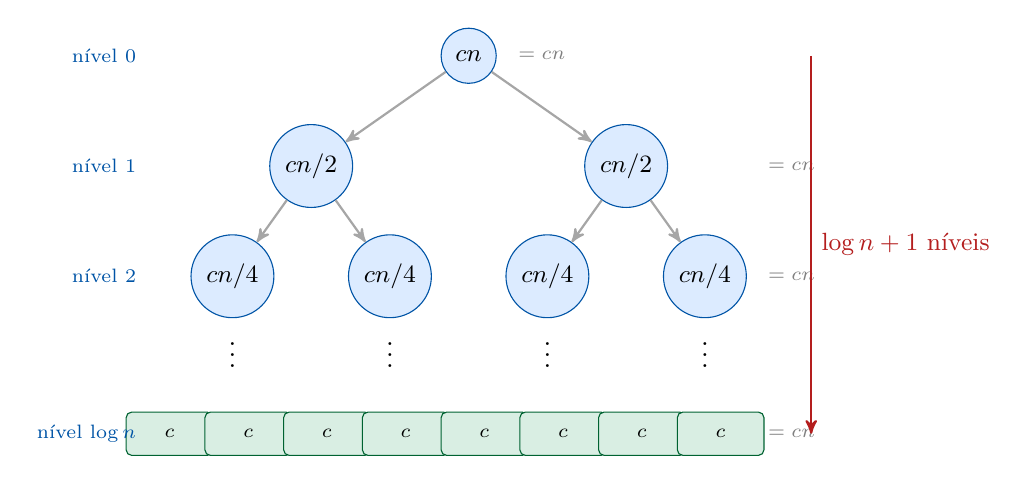
\begin{tikzpicture}[node distance=0.3cm]
    % Nível 0
    \node[treenode] (r) at (4, 5) {$cn$};
    \node[font=\scriptsize, color=gray, right=0.15cm of r] {$= cn$};

    % Nível 1
    \node[treenode] (l1) at (2, 3.6) {$cn/2$};
    \node[treenode] (r1) at (6, 3.6) {$cn/2$};
    \node[font=\scriptsize, color=gray] at (8.1, 3.6) {$= cn$};

    % Nível 2
    \node[treenode] (ll2) at (1,   2.2) {$cn/4$};
    \node[treenode] (lr2) at (3,   2.2) {$cn/4$};
    \node[treenode] (rl2) at (5,   2.2) {$cn/4$};
    \node[treenode] (rr2) at (7,   2.2) {$cn/4$};
    \node[font=\scriptsize, color=gray] at (8.1, 2.2) {$= cn$};

    % Pontos de continuação
    \node at (1,   1.3) {$\vdots$};
    \node at (3,   1.3) {$\vdots$};
    \node at (5,   1.3) {$\vdots$};
    \node at (7,   1.3) {$\vdots$};

    % Folhas (8 folhas uniformes)
    \foreach \x in {0.2, 1.2, 2.2, 3.2, 4.2, 5.2, 6.2, 7.2} {
      \node[treeleaf] at (\x, 0.2) {$c$};
    }
    \node[font=\scriptsize, color=gray] at (8.1, 0.2) {$= cn$};

    % Setas
    \draw[treearrow] (r) -- (l1);
    \draw[treearrow] (r) -- (r1);
    \draw[treearrow] (l1) -- (ll2);
    \draw[treearrow] (l1) -- (lr2);
    \draw[treearrow] (r1) -- (rl2);
    \draw[treearrow] (r1) -- (rr2);

    % Rótulo de profundidade
    \node[font=\scriptsize\color{UFSBlue}, left] at (-0.1, 5)   {nível 0};
    \node[font=\scriptsize\color{UFSBlue}, left] at (-0.1, 3.6) {nível 1};
    \node[font=\scriptsize\color{UFSBlue}, left] at (-0.1, 2.2) {nível 2};
    \node[font=\scriptsize\color{UFSBlue}, left] at (-0.1, 0.2) {nível $\log n$};

    % Seta de total (custo por nível)
    \draw[->, >=stealth', thick, color=alertRed]
          (8.35, 5) -- (8.35, 0.2)
          node[midway, right, font=\small, color=alertRed]
               {$\log n + 1$ níveis};
  \end{tikzpicture}}%

  \vspace{4pt}
  \[
    T(n) = cn \cdot (\log n + 1) = \Theta(n \log n)
  \]
\end{frame}

\begin{frame}{Análise dos Casos}
  \begin{block}{Merge Sort — todos os casos são iguais}
    \begin{center}
      \renewcommand{\arraystretch}{1.3}
      \begin{tabular}{lccc}
        \hline
        \textbf{Caso} & \textbf{Divisão} & \textbf{Merge} & \textbf{Total} \\
        \hline
        Melhor   & $\Theta(\log n)$ & $\Theta(n)$ por nível & $\Theta(n \log n)$ \\
        Médio    & $\Theta(\log n)$ & $\Theta(n)$ por nível & $\Theta(n \log n)$ \\
        Pior     & $\Theta(\log n)$ & $\Theta(n)$ por nível & $\Theta(n \log n)$ \\
        \hline
      \end{tabular}
    \end{center}
  \end{block}

  \vspace{6pt}
  \begin{alertblock}{Desvantagem}
    \textbf{Espaço auxiliar}: $\Theta(n)$ — não é \emph{in-place}\\
    (as cópias $L$ e $R$ no \textsc{Merge} exigem memória extra)
  \end{alertblock}
\end{frame}

\begin{frame}{Comparação: Insertion Sort vs.\ Merge Sort}
  \centering
  \renewcommand{\arraystretch}{1.4}
  \begin{tabular}{lcc}
    \hline
    \textbf{Propriedade} & \textbf{Insertion Sort} & \textbf{Merge Sort} \\
    \hline
    Pior caso    & $\Theta(n^2)$   & $\Theta(n \log n)$ \\
    Melhor caso  & $\Theta(n)$     & $\Theta(n \log n)$ \\
    Estável      & Sim             & Sim \\
    In-place     & Sim             & Não \\
    Uso prático  & $n$ pequeno     & $n$ grande \\
    \hline
  \end{tabular}
\end{frame}

% =============================================================
% QUICK SORT
% =============================================================
\part{Quick Sort}
\section{Quick Sort}

\begin{frame}{Quick Sort — Ideia Central}
  \begin{columns}[T]
    \begin{column}{0.54\textwidth}
      \begin{block}{Divisão e Conquista (ao contrário)}
        \begin{enumerate}
          \item \textbf{Escolher} um elemento \emph{pivô} $x$
          \item \textbf{Particionar}: rearranjar $A$ em\\
                $[\underbrace{\leq x}_{\text{esq}}]\;[x]\;[\underbrace{\geq x}_{\text{dir}}]$
          \item \textbf{Conquistar}: ordenar recursivamente esquerda e direita
          \item \textbf{Combinar}: nada a fazer!
        \end{enumerate}
      \end{block}
    \end{column}
    \begin{column}{0.42\textwidth}
      \begin{exampleblock}{Características}
        \begin{itemize}
          \item \textbf{In-place}: $O(\log n)$ pilha
          \item Caso médio: $\Theta(n \log n)$
          \item Pior caso: $\Theta(n^2)$
          \item Na prática: muito eficiente
        \end{itemize}
      \end{exampleblock}
    \end{column}
  \end{columns}
\end{frame}

\begin{frame}[fragile]{Quick Sort — pseudocódigo}
  \begin{algorithm}[H]
    \caption{\textsc{QuickSort}$(A, p, r)$}
    \begin{algorithmic}[1]
      \If{$p < r$}
        \State $q \gets \textsc{Partition}(A, p, r)$
        \State \textsc{QuickSort}$(A, p, q - 1)$
        \State \textsc{QuickSort}$(A, q + 1, r)$
      \EndIf
    \end{algorithmic}
  \end{algorithm}

  \vspace{8pt}
  \begin{itemize}
    \item O pivô termina na posição \emph{correta} após \textsc{Partition}
    \item Chamada inicial: \textsc{QuickSort}$(A, 1, n)$
    \item Todo o trabalho está em \textsc{Partition} — $\Theta(n)$
  \end{itemize}
\end{frame}

\begin{frame}[fragile]{Partição de Lomuto}
  \begin{columns}[T]
    \begin{column}{0.5\textwidth}
      \begin{algorithm}[H]
        \caption{\textsc{Partition}$(A, p, r)$}
        \begin{algorithmic}[1]
          \State $x \gets A[r]$ \Comment{pivô = último}
          \State $i \gets p - 1$
          \For{$j \gets p$ \textbf{to} $r - 1$}
            \If{$A[j] \leq x$}
              \State $i \gets i + 1$
              \State \textbf{trocar} $A[i] \leftrightarrow A[j]$
            \EndIf
          \EndFor
          \State \textbf{trocar} $A[i{+}1] \leftrightarrow A[r]$
          \State \Return $i + 1$
        \end{algorithmic}
      \end{algorithm}
    \end{column}
    \begin{column}{0.46\textwidth}
      \begin{block}{Invariante do loop}
        Ao início de cada iteração $j$:
        \begin{itemize}
          \item $A[p \ldots i] \leq x$
          \item $A[i{+}1 \ldots j{-}1] > x$
          \item $A[r] = x$ (pivô)
        \end{itemize}
      \end{block}
      \vspace{4pt}
      Complexidade: $\Theta(r - p)$
    \end{column}
  \end{columns}
\end{frame}

\begin{frame}[shrink=5]{Visualização da Partição (Lomuto)}
  \centering
  {\small Particionando $A = [2, 8, 7, 1, 3, 5, 6, 4]$, pivô $= 4$}

  \vspace{6pt}
  \resizebox{0.9\textwidth}{!}{%
  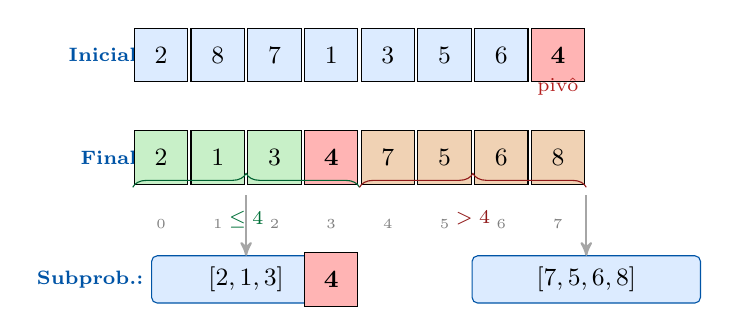
\begin{tikzpicture}
    % --- estado inicial ---
    \node[font=\scriptsize\bfseries, color=UFSBlue, left] at (-0.1, 3.4) {Inicial:};
    \foreach \v/\k in {2/0,8/1,7/2,1/3,3/4,5/5,6/6,4/7} {
      \ifnum\k=7
        \node[cellpivot] at (\k*0.72, 3.4) {\v};
      \else
        \node[cell]      at (\k*0.72, 3.4) {\v};
      \fi
    }
    \node[font=\scriptsize, color=alertRed] at (7*0.72, 3.0) {pivô};

    % --- após particionar ---
    \node[font=\scriptsize\bfseries, color=UFSBlue, left] at (-0.1, 2.1) {Final:};
    % ≤ 4
    \foreach \v/\k in {2/0,1/1,3/2} {
      \node[celllt] at (\k*0.72, 2.1) {\v};
    }
    % pivô no lugar certo
    \node[cellpivot] at (3*0.72, 2.1) {4};
    % > 4
    \foreach \v/\k in {7/4,5/5,6/6,8/7} {
      \node[cellgt] at (\k*0.72, 2.1) {\v};
    }

    % rótulos de região
    \draw[decorate, decoration={brace,amplitude=5pt}, color=sicpGreen!70!black]
         (-0.36+0*0.72, 1.72) -- (-0.36+4*0.72, 1.72)
         node[midway, below=5pt, font=\scriptsize, color=sicpGreen!80!black]
              {$\leq 4$};
    \draw[decorate, decoration={brace,amplitude=5pt}, color=alertRed!80!black]
         (-0.36+4*0.72, 1.72) -- (-0.36+8*0.72, 1.72)
         node[midway, below=5pt, font=\scriptsize, color=alertRed!80!black]
              {$> 4$};

    % índices
    \foreach \k in {0,...,7} {
      \node[font=\tiny, color=gray] at (\k*0.72, 1.25) {\k};
    }

    % --- subproblemas ---
    \node[font=\scriptsize\bfseries, color=UFSBlue, left] at (-0.1, 0.55) {Subprob.:};
    \node[rectnode, minimum width=2.4cm] at (1.08, 0.55) {$[2,1,3]$};
    \node[cellpivot, minimum width=0.68cm] at (3*0.72, 0.55) {4};
    \node[rectnode, minimum width=2.9cm] at (5.4, 0.55) {$[7,5,6,8]$};

    \draw[treearrow] (1.08, 1.72-0.1) -- (1.08, 0.85);
    \draw[treearrow] (5.4,  1.72-0.1) -- (5.4,  0.85);
  \end{tikzpicture}}%
\end{frame}

\begin{frame}[shrink=8]{Pior Caso: $\Theta(n^2)$}
  \begin{columns}[T]
    \begin{column}{0.48\textwidth}
      \begin{alertblock}{Quando ocorre?}
        Pivô é sempre o \textbf{menor} ou \textbf{maior} elemento:\\
        partição desequilibrada $[\ ] \mid x \mid [n{-}1]$
      \end{alertblock}
      \vspace{6pt}
      \textbf{Recorrência:}
      \[
        T(n) = T(0) + T(n{-}1) + \Theta(n)
      \]
      \[
        T(n) = \Theta(n^2)
      \]
      \vspace{4pt}
      {\small Ocorre para entrada já ordenada\\com pivô = último elemento.}
    \end{column}
    \begin{column}{0.48\textwidth}
      \centering
      \resizebox{0.95\columnwidth}{!}{%
      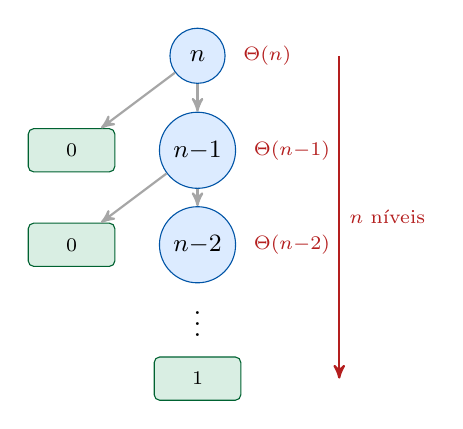
\begin{tikzpicture}
        % Árvore degenerada
        \node[treenode] (n0) at (2.0, 5.0) {$n$};
        \node[treeleaf] (e0) at (0.4, 3.8) {$0$};
        \node[treenode] (n1) at (2.0, 3.8) {$n{-}1$};
        \node[treeleaf] (e1) at (0.4, 2.6) {$0$};
        \node[treenode] (n2) at (2.0, 2.6) {$n{-}2$};
        \node at (2.0, 1.7) {$\vdots$};
        \node[treeleaf] (nk) at (2.0, 0.9) {$1$};

        \draw[treearrow] (n0) -- (e0);
        \draw[treearrow] (n0) -- (n1);
        \draw[treearrow] (n1) -- (e1);
        \draw[treearrow] (n1) -- (n2);

        % Custos à direita
        \node[font=\scriptsize, color=alertRed, right=0.1cm of n0] {$\Theta(n)$};
        \node[font=\scriptsize, color=alertRed, right=0.1cm of n1] {$\Theta(n{-}1)$};
        \node[font=\scriptsize, color=alertRed, right=0.1cm of n2] {$\Theta(n{-}2)$};

        \draw[worstarrow] (3.8, 5.0) -- (3.8, 0.9)
              node[midway, right, font=\scriptsize, color=alertRed]
                   {$n$ níveis};
      \end{tikzpicture}}%
    \end{column}
  \end{columns}
\end{frame}

\begin{frame}[shrink=5]{Melhor Caso e Caso Médio}
  \begin{columns}[T]
    \begin{column}{0.46\textwidth}
      \begin{block}{Melhor caso}
        Partição sempre \textbf{equilibrada} $(n/2 \mid n/2)$:
        \[
          T(n) = 2T(n/2) + \Theta(n) = \Theta(n \log n)
        \]
        (mesma recorrência do Merge Sort)
      \end{block}
    \end{column}
    \begin{column}{0.50\textwidth}
      \begin{block}{Caso médio — intuição}
        Se partições são $9:1$ (``ruim''):
        \[
          T(n) = T(9n/10) + T(n/10) + \Theta(n)
        \]
        Mesmo assim: $\Theta(n \log n)$!
      \end{block}
    \end{column}
  \end{columns}

  \vspace{8pt}
  \begin{exampleblock}{Resultado principal (CLRS Teorema 7.4)}
    Assumindo todas as permutações igualmente prováveis,
    o tempo \textbf{esperado} do Quick Sort é $\Theta(n \log n)$.
    O número esperado de comparações é $\approx 1{,}386\,n \log n$.
  \end{exampleblock}
\end{frame}

\begin{frame}[fragile,shrink=8]{Quick Sort Randomizado}
  \begin{columns}[T]
    \begin{column}{0.50\textwidth}
      \begin{algorithm}[H]
        \caption{\textsc{RandPartition}$(A, p, r)$}
        \begin{algorithmic}[1]
          \State $i \gets \textsc{Random}(p, r)$
          \State \textbf{trocar} $A[i] \leftrightarrow A[r]$
          \State \Return \textsc{Partition}$(A, p, r)$
        \end{algorithmic}
      \end{algorithm}

      \vspace{8pt}
      \begin{algorithm}[H]
        \caption{\textsc{RandQuickSort}$(A, p, r)$}
        \begin{algorithmic}[1]
          \If{$p < r$}
            \State $q \gets \textsc{RandPartition}(A, p, r)$
            \State \textsc{RandQuickSort}$(A, p, q{-}1)$
            \State \textsc{RandQuickSort}$(A, q{+}1, r)$
          \EndIf
        \end{algorithmic}
      \end{algorithm}
    \end{column}
    \begin{column}{0.46\textwidth}
      \begin{block}{Por que randomizar?}
        \begin{itemize}
          \item Elimina dependência da entrada
          \item Pior caso ainda $\Theta(n^2)$, mas com probabilidade
                \emph{exponencialmente pequena}
          \item Tempo esperado: $\Theta(n \log n)$ para \textbf{qualquer} entrada
        \end{itemize}
      \end{block}
      \vspace{6pt}
      \begin{exampleblock}{Na prática}
        Alternativas ao pivô aleatório:\\
        \textbf{Mediana de 3}: $A[p]$, $A[\lfloor(p{+}r)/2\rfloor]$, $A[r]$
      \end{exampleblock}
    \end{column}
  \end{columns}
\end{frame}

\begin{frame}{Resumo: Merge Sort vs.\ Quick Sort}
  \centering
  \renewcommand{\arraystretch}{1.4}
  \begin{tabular}{lcc}
    \hline
    \textbf{Propriedade} & \textbf{Merge Sort} & \textbf{Quick Sort} \\
    \hline
    Pior caso     & $\Theta(n \log n)$ & $\Theta(n^2)$ \\
    Caso médio    & $\Theta(n \log n)$ & $\Theta(n \log n)$ \\
    In-place      & Não & Sim \\
    Estável       & Sim & Não \\
    Memória extra & $\Theta(n)$ & $O(\log n)$ \\
    \hline
  \end{tabular}
\end{frame}

% =============================================================
% LIMITE INFERIOR
% =============================================================
\part{Limite Inferior}
\section{Limite Inferior}

\begin{frame}{O que é uma Árvore de Decisão?}
  \begin{block}{Definição}
    Uma \textbf{árvore de decisão} modela o comportamento de qualquer algoritmo de
    ordenação por comparação sobre uma entrada de tamanho $n$.
  \end{block}

  \medskip
  \begin{itemize}
    \item Cada \textbf{nó interno} representa uma comparação $a_i : a_j$
    \item O resultado da comparação ($\leq$ ou $>$) determina o ramo seguido
    \item Cada \textbf{folha} corresponde a uma permutação final (ordenação) possível
    \item A \textbf{profundidade} de uma folha = número de comparações naquele caminho
    \item O \textbf{pior caso} = \textbf{altura} da árvore
  \end{itemize}
\end{frame}

\begin{frame}{Exemplo: Árvore de Decisão para $n=3$}
  \begin{center}
  \resizebox{0.9\textwidth}{!}{%
  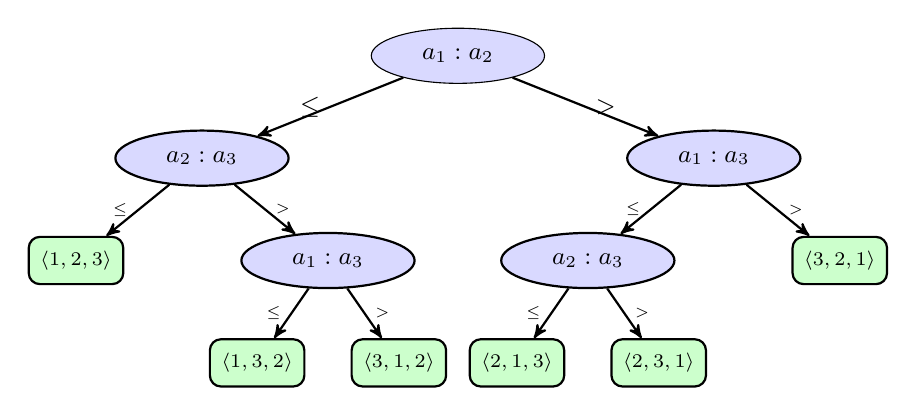
\begin{tikzpicture}[level distance=1.3cm,
      level 1/.style={sibling distance=6.5cm},
      level 2/.style={sibling distance=3.2cm},
      level 3/.style={sibling distance=1.8cm}]

    \node[decnode] {$a_1 : a_2$}
      child[treeedge] {
        node[decnode] {$a_2 : a_3$}
        child[treeedge] {
          node[leafnode] {$\langle 1,2,3\rangle$}
          edge from parent node[left, font=\tiny] {$\leq$}
        }
        child[treeedge] {
          node[decnode] {$a_1 : a_3$}
          child[treeedge] {
            node[leafnode] {$\langle 1,3,2\rangle$}
            edge from parent node[left, font=\tiny] {$\leq$}
          }
          child[treeedge] {
            node[leafnode] {$\langle 3,1,2\rangle$}
            edge from parent node[right, font=\tiny] {$>$}
          }
          edge from parent node[right, font=\tiny] {$>$}
        }
        edge from parent node[left, font=\small] {$\leq$}
      }
      child[treeedge] {
        node[decnode] {$a_1 : a_3$}
        child[treeedge] {
          node[decnode] {$a_2 : a_3$}
          child[treeedge] {
            node[leafnode] {$\langle 2,1,3\rangle$}
            edge from parent node[left, font=\tiny] {$\leq$}
          }
          child[treeedge] {
            node[leafnode] {$\langle 2,3,1\rangle$}
            edge from parent node[right, font=\tiny] {$>$}
          }
          edge from parent node[left, font=\tiny] {$\leq$}
        }
        child[treeedge] {
          node[leafnode] {$\langle 3,2,1\rangle$}
          edge from parent node[right, font=\tiny] {$>$}
        }
        edge from parent node[right, font=\small] {$>$}
      };
  \end{tikzpicture}%
  }
  \end{center}
  \vspace{-0.3cm}
  {\small Altura $= 3$; todas as $3! = 6$ permutações aparecem como folhas.}
\end{frame}

\begin{frame}[shrink=5]{Por que a Árvore Precisa de Pelo Menos $n!$ Folhas?}
  \begin{alertblock}{Argumento de Corretude}
    Um algoritmo de ordenação correto deve ser capaz de produzir \textbf{qualquer} uma das
    $n!$ permutações possíveis da entrada.
  \end{alertblock}

  \medskip
  \begin{itemize}
    \item Para $n$ elementos, existem $n! = n \times (n{-}1) \times \cdots \times 1$ ordenações possíveis
    \item Se dois inputs distintos levam à mesma folha $\Rightarrow$ o algoritmo produz a mesma saída para ambos $\Rightarrow$ \textbf{incorreto} para ao menos um deles
    \item Portanto, cada permutação deve corresponder a \textbf{ao menos uma folha distinta}
  \end{itemize}

  \medskip
  \begin{block}{Conclusão}
    \[
      \text{número de folhas} \;\geq\; n!
    \]
  \end{block}
\end{frame}

\begin{frame}{Visualização: Folhas vs.\ Permutações}
  \begin{columns}[T]
    \begin{column}{0.48\textwidth}
      \textbf{Árvore binária de altura $h$:}
      \begin{itemize}
        \item Tem no máximo $2^h$ folhas
        \item Cada folha = 1 resposta possível
      \end{itemize}
      \vspace{0.4cm}
      \resizebox{\columnwidth}{!}{%
      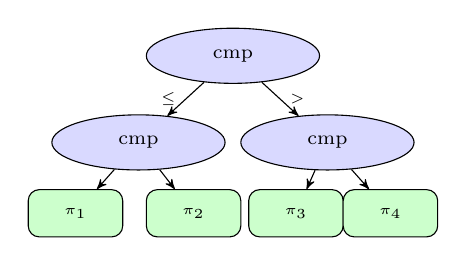
\begin{tikzpicture}
        \node[decnode, font=\scriptsize] (r) at (2,2) {cmp};
        \node[decnode, font=\scriptsize] (l) at (0.8,0.9) {cmp};
        \node[decnode, font=\scriptsize] (rr) at (3.2,0.9) {cmp};
        \node[leafnode, font=\tiny] (ll) at (0,0) {$\pi_1$};
        \node[leafnode, font=\tiny] (lr) at (1.5,0) {$\pi_2$};
        \node[leafnode, font=\tiny] (rl) at (2.8,0) {$\pi_3$};
        \node[leafnode, font=\tiny] (rro) at (4.0,0) {$\pi_4$};
        \draw[thinedge] (r) -- (l) node[midway,left,font=\tiny]{$\leq$};
        \draw[thinedge] (r) -- (rr) node[midway,right,font=\tiny]{$>$};
        \draw[thinedge] (l) -- (ll);
        \draw[thinedge] (l) -- (lr);
        \draw[thinedge] (rr) -- (rl);
        \draw[thinedge] (rr) -- (rro);
      \end{tikzpicture}}%
    \end{column}
    \begin{column}{0.48\textwidth}
      \textbf{Restrição de corretude:}
      \[
        2^h \;\geq\; n!
      \]
      \vspace{0.3cm}
      \begin{tabular}{c|r|c}
        $n$ & $n!$ & $h_{\min}$ \\\hline
        3 & 6   & 3 \\
        4 & 24  & 5 \\
        5 & 120 & 7 \\
        8 & 40320 & 16 \\
      \end{tabular}
    \end{column}
  \end{columns}
\end{frame}

\begin{frame}[shrink=10]{Limite Inferior para a Altura}
  \begin{block}{Teorema}
    Qualquer árvore de decisão que ordena $n$ elementos tem altura $h \geq \lceil \log_2(n!) \rceil$.
  \end{block}

  \medskip
  \textbf{Prova:}
  \begin{enumerate}
    \item Uma árvore binária de altura $h$ possui no máximo $2^h$ folhas
    \item A árvore precisa de pelo menos $n!$ folhas (slide anterior)
    \item Portanto:
      \[
        2^h \;\geq\; n!
        \;\implies\;
        h \;\geq\; \log_2(n!)
      \]
    \item Como $h$ é inteiro: $h \geq \lceil \log_2(n!) \rceil$ \qquad $\blacksquare$
  \end{enumerate}

  \begin{alertblock}{Interpretação}
    O \textbf{pior caso} de qualquer algoritmo de ordenação por comparação requer
    pelo menos $\lceil \log_2(n!) \rceil$ comparações.
  \end{alertblock}
\end{frame}

\begin{frame}[shrink=5]{Aproximação de Stirling}
  \begin{block}{Fórmula de Stirling}
    \[
      n! \;\approx\; \sqrt{2\pi n}\left(\frac{n}{e}\right)^n
      \qquad \text{(para $n$ grande)}
    \]
  \end{block}

  \medskip
  Aplicando $\log_2$:
  \[
    \log_2(n!)
    \;\approx\;
    \frac{1}{2}\log_2(2\pi n) + n\log_2 n - n\log_2 e
  \]

  \medskip
  O termo dominante é $n \log_2 n$, então:
  \[
    \log_2(n!) \;=\; \Theta(n \log n)
  \]

  \begin{exampleblock}{Prova direta simples (lower bound)}
    \[
      \log_2(n!)
      = \sum_{k=1}^{n}\log_2 k
      \;\geq\;
      \sum_{k=\lceil n/2 \rceil}^{n}\log_2 k
      \;\geq\;
      \frac{n}{2}\log_2\!\left(\frac{n}{2}\right)
      = \Omega(n\log n)
    \]
  \end{exampleblock}
\end{frame}

\begin{frame}[shrink=5]{Visualização: Crescimento de $\log_2(n!)$}
  \begin{columns}[T]
    \begin{column}{0.54\textwidth}
      \resizebox{\columnwidth}{!}{%
      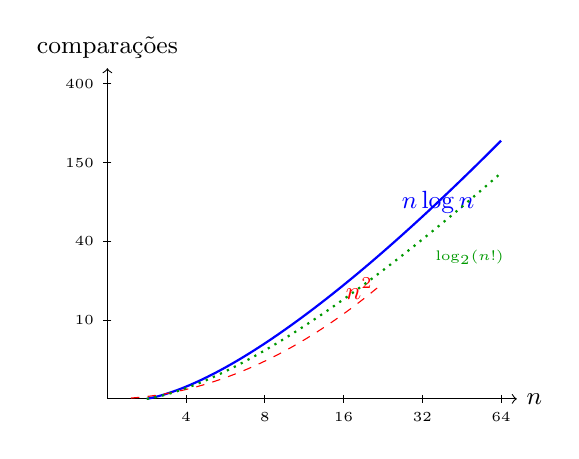
\begin{tikzpicture}
        % eixos
        \draw[->] (0,0) -- (5.2,0) node[right,font=\small] {$n$};
        \draw[->] (0,0) -- (0,4.2) node[above,font=\small] {comparações};
        % ticks eixo x
        \foreach \x/\lbl in {1/4, 2/8, 3/16, 4/32, 5/64} {
          \draw (\x,0.05) -- (\x,-0.05) node[below,font=\tiny] {\lbl};
        }
        % ticks eixo y
        \foreach \y/\lbl in {1/10, 2/40, 3/150, 4/400} {
          \draw (0.05,\y) -- (-0.05,\y) node[left,font=\tiny] {\lbl};
        }
        % curva n log n (aproximada)
        \draw[blue, thick, domain=0.5:5, samples=60]
          plot (\x, {0.8*\x*ln(\x+0.5)/ln(2)/3});
        \node[blue, font=\small] at (4.2,2.5) {$n\log n$};
        % curva n^2 (aproximada)
        \draw[red, dashed, domain=0.3:3.5, samples=40]
          plot (\x, {0.12*\x*\x});
        \node[red, font=\small] at (3.2,1.4) {$n^2$};
        % linha limite inferior
        \draw[green!60!black, dotted, thick, domain=0.5:5, samples=60]
          plot (\x, {0.7*\x*ln(\x+0.5)/ln(2)/3});
        \node[green!60!black, font=\tiny] at (4.6,1.8) {$\log_2(n!)$};
      \end{tikzpicture}%
      }
    \end{column}
    \begin{column}{0.42\textwidth}
      \textbf{Tabela de $\lfloor\log_2(n!)\rfloor$:}
      \medskip

      \begin{tabular}{c|r|r}
        $n$ & $n!$ & $\lfloor\log_2(n!)\rfloor$ \\\hline
        4  & 24        & 4  \\
        8  & 40.320    & 15 \\
        16 & $\approx 2{\times}10^{13}$ & 44 \\
        32 & $\approx 2{\times}10^{35}$ & 117\\
      \end{tabular}

      \medskip
      \textbf{Cresce como $\Theta(n\log n)$!}
    \end{column}
  \end{columns}
\end{frame}

\begin{frame}[shrink=10]{Teorema: Limite Inferior $\Omega(n \log n)$}
  \begin{block}{Teorema (CLRS, Cap.\ 8)}
    Qualquer algoritmo de ordenação por comparação requer $\Omega(n \log n)$
    comparações no pior caso.
  \end{block}

  \medskip
  \textbf{Resumo da prova:}
  \begin{enumerate}
    \item Todo algoritmo de ordenação por comparação pode ser modelado por uma árvore de decisão
    \item A árvore deve ter $\geq n!$ folhas (corretude)
    \item Uma árvore binária com $\geq n!$ folhas tem altura $h \geq \log_2(n!)$
    \item Pela aproximação de Stirling: $\log_2(n!) = \Omega(n\log n)$
    \item Logo $h = \Omega(n\log n)$ \qquad $\blacksquare$
  \end{enumerate}

  \begin{alertblock}{Corolário}
    HeapSort (visto em aula anterior) e MergeSort são \textbf{ótimos assintoticamente}: ambos rodam em $\Theta(n\log n)$.
  \end{alertblock}
\end{frame}

% =============================================================
% COUNTING SORT
% =============================================================
\part{Counting Sort}
\section{Counting Sort}

\begin{frame}{Por que ir além de $\Omega(n \log n)$?}
  \begin{block}{Limite inferior para ordenação por comparação}
    Qualquer algoritmo baseado em comparações precisa de $\Omega(n \log n)$
    comparações no pior caso.
  \end{block}
  \vspace{0.3cm}
  \begin{itemize}
    \item Se soubermos \textbf{mais} sobre os dados, podemos ordenar mais rápido.
    \item \textbf{Counting Sort} não usa comparações entre elementos.
    \item Assume que os elementos são inteiros no intervalo $[0,\, k]$.
    \item Complexidade: $\Theta(n + k)$ — linear quando $k = O(n)$.
  \end{itemize}
  \vspace{0.3cm}
  \begin{exampleblock}{Quando usar?}
    Chaves inteiras em intervalo pequeno: idades, notas (0–100),
    caracteres ASCII, dígitos decimais.
  \end{exampleblock}
\end{frame}

\begin{frame}{Quando usar o Counting Sort?}
  \begin{columns}[T]
    \begin{column}{0.50\textwidth}
      \textbf{\checkmark\ Favorável}
      \begin{itemize}
        \item Chaves inteiras não-negativas
        \item Intervalo $k = O(n)$
        \item Necessidade de estabilidade
        \item Sub-rotina do Radix Sort
      \end{itemize}
    \end{column}
    \begin{column}{0.50\textwidth}
      \textbf{$\times$\ Desfavorável}
      \begin{itemize}
        \item Chaves reais ou strings
        \item $k \gg n$ (intervalo enorme)
        \item Memória muito restrita ($\Theta(n+k)$)
        \item Dados com distribuição desconhecida
      \end{itemize}
    \end{column}
  \end{columns}
  \vspace{0.5cm}
  \begin{center}
  \resizebox{0.85\textwidth}{!}{%
  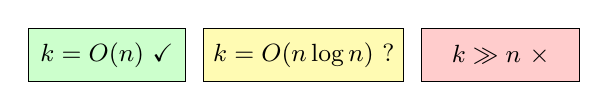
\begin{tikzpicture}
    \node[cell, fill=green!20,  minimum width=2cm] at (0,0)   {$k=O(n)$ \checkmark};
    \node[cell, fill=yellow!30, minimum width=2cm] at (2.5,0) {$k=O(n\log n)$ ?};
    \node[cell, fill=red!20,    minimum width=2cm] at (5,0)   {$k \gg n$ $\times$};
  \end{tikzpicture}}%
  \end{center}
\end{frame}

\begin{frame}[fragile]{Counting Sort — Pseudocódigo}
  \textbf{\textsc{CountingSort}}$(A[1..n],\; B[1..n],\; k)$\\
  \emph{Entrada:} $A[i]\in[0,k]$;\quad \emph{Saída:} $B$ ordenado
\begin{lstlisting}[basicstyle=\ttfamily\scriptsize]
// Passo 1: contar ocorrencias  Theta(k) + Theta(n)
C[0..k] <- 0
for j = 1 to n do
    C[A[j]] += 1

// Passo 2: acumular prefixo   Theta(k)
for i = 1 to k do
    C[i] += C[i-1]

// Passo 3: espalhar (traz p/ frente)  Theta(n)
for j = n downto 1 do
    B[C[A[j]]] <- A[j]
    C[A[j]] -= 1
\end{lstlisting}
  \textbf{Três varreduras:} contar $\to$ acumular $\to$ espalhar.
\end{frame}

\begin{frame}[shrink]{Visualização: Array de Contagem (Passo 1 e 2)}

  \textbf{Entrada} $A = [2,5,3,0,2,3,0,3]$ \quad ($n=8$,\ $k=5$)

  \vspace{0.1cm}
  \textbf{Passo 1 — Contar:}
  \begin{center}
    \resizebox{0.8\textwidth}{!}{
      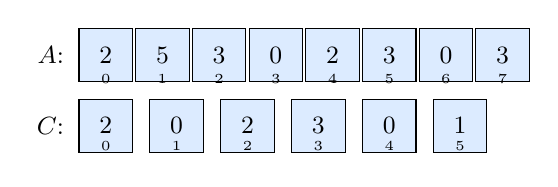
\begin{tikzpicture}
        \foreach \val/\i in {2/0,5/1,3/2,0/3,2/4,3/5,0/6,3/7}{
          \node[cell] at (\i*0.72, 0.9) {\val};
          \node[font=\tiny] at (\i*0.72, 0.6) {\i};
        }
        \node[left=3pt,font=\small] at (-0.3,0.9) {$A$:};
        \foreach \val/\i in {2/0,0/1,2/2,3/3,0/4,1/5}{
          \node[cell] at (\i*0.9, 0) {\val};
          \node[font=\tiny] at (\i*0.9,-0.25) {\i};
        }
        \node[left=3pt,font=\small] at (-0.3,0) {$C$:};
      \end{tikzpicture}
    }
  \end{center}

  \vspace{-0.1cm}
  \textbf{Passo 2 — Acumular prefixo} ($C'[i] = |\{j : A[j] \le i\}|$):
  \begin{center}
    \resizebox{0.6\textwidth}{!}{
      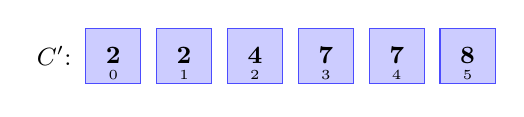
\begin{tikzpicture}
        \foreach \val/\i in {2/0,2/1,4/2,7/3,7/4,8/5}{
          \node[cellh] at (\i*0.9, 0) {\val};
          \node[font=\tiny] at (\i*0.9,-0.25) {\i};
        }
        \node[left=3pt,font=\small] at (-0.3,0) {$C'$:};
      \end{tikzpicture}
    }
  \end{center}

  \vspace{-0.1cm}
  \textbf{Passo 3 — Saída $B$ (espalhar de trás para frente):}
  \begin{center}
    \resizebox{0.8\textwidth}{!}{
      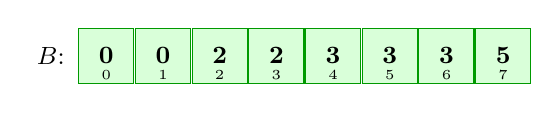
\begin{tikzpicture}
        \foreach \val/\i in {0/0,0/1,2/2,2/3,3/4,3/5,3/6,5/7}{
          \node[cellout] at (\i*0.72, 0) {\val};
          \node[font=\tiny] at (\i*0.72,-0.25) {\i};
        }
        \node[left=3pt,font=\small] at (-0.3,0) {$B$:};
      \end{tikzpicture}
    }
  \end{center}
\end{frame}

\begin{frame}[shrink]{Invariante do Loop — Fase de Espalhamento}
  \begin{block}{Invariante (início de cada iteração do 3.º \textbf{for})}
    Para cada valor $v \in [0,k]$,\ $C[v]$ contém o número de elementos de
    $A[1..j]$ menores ou iguais a $v$ que \textbf{ainda não foram colocados} em $B$.
    Equivalentemente, $B[C[v]+1..(\text{posição original de }v)]$ está corretamente
    preenchido com os $n - j$ elementos já processados.
  \end{block}

  \vspace{0.4cm}
  \begin{columns}[T]
    \begin{column}{0.48\textwidth}
      \textbf{Inicialização ($j=n$):}\\
      $C[v]$ = número de elementos $\le v$
      em $A$ inteiro. Correto pois nenhum
      elemento foi colocado em $B$ ainda.
    \end{column}
    \begin{column}{0.48\textwidth}
      \textbf{Manutenção:}\\
      Ao processar $A[j]$: colocamos
      $A[j]$ em $B[C[A[j]]]$ e decrementamos
      $C[A[j]]$, mantendo o invariante para
      a próxima iteração.
    \end{column}
  \end{columns}

  \vspace{0.3cm}
  \begin{exampleblock}{Término}
    Quando $j=0$, todo $A[1..n]$ foi processado e $B$ está ordenado.
  \end{exampleblock}
\end{frame}

\begin{frame}[shrink]{Análise de Complexidade: $\Theta(n+k)$}
  \begin{block}{Contando operações}
    \begin{tabular}{llr}
      \hline
      Etapa & Operação & Custo \\
      \hline
      Inicializar $C$ & $k+1$ atribuições & $\Theta(k)$ \\
      Contar (\textbf{1.º} for) & $n$ incrementos & $\Theta(n)$ \\
      Acumular (\textbf{2.º} for) & $k$ somas & $\Theta(k)$ \\
      Espalhar (\textbf{3.º} for) & $n$ escritas & $\Theta(n)$ \\
      \hline
      \textbf{Total} & & $\Theta(n+k)$ \\
      \hline
    \end{tabular}
  \end{block}

  \vspace{0.3cm}
  \begin{columns}[T]
    \begin{column}{0.55\textwidth}
      \begin{itemize}
        \item \textbf{Tempo:} $\Theta(n+k)$
        \item \textbf{Espaço:} $\Theta(n+k)$ (arrays $B$ e $C$)
        \item Se $k = O(n)$: tempo \textbf{linear} $\Theta(n)$
        \item Não é baseado em comparação $\Rightarrow$\\
              não viola o limite $\Omega(n \log n)$
      \end{itemize}
    \end{column}
    \begin{column}{0.42\textwidth}
      \begin{center}
      \resizebox{\columnwidth}{!}{%
      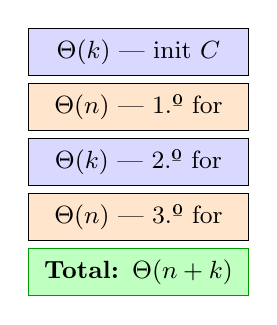
\begin{tikzpicture}
        \node[cell, fill=blue!15, minimum width=2.8cm, minimum height=0.6cm]
          at (0,1.6) {$\Theta(k)$ — init $C$};
        \node[cell, fill=orange!20, minimum width=2.8cm, minimum height=0.6cm]
          at (0,0.9) {$\Theta(n)$ — 1.º for};
        \node[cell, fill=blue!15, minimum width=2.8cm, minimum height=0.6cm]
          at (0,0.2) {$\Theta(k)$ — 2.º for};
        \node[cell, fill=orange!20, minimum width=2.8cm, minimum height=0.6cm]
          at (0,-0.5) {$\Theta(n)$ — 3.º for};
        \node[cell, fill=green!25, minimum width=2.8cm, minimum height=0.6cm,
              draw=green!60!black]
          at (0,-1.2) {\textbf{Total: }$\Theta(n+k)$};
      \end{tikzpicture}}%
      \end{center}
    \end{column}
  \end{columns}
\end{frame}

\begin{frame}[shrink]{Estabilidade do Counting Sort}
  \begin{block}{Definição — Algoritmo estável}
    Um algoritmo de ordenação é \textbf{estável} se elementos com chaves iguais
    aparecem na saída na \textbf{mesma ordem relativa} em que aparecem na entrada.
  \end{block}

  \vspace{0.3cm}
  \textbf{Por que o Counting Sort é estável?}
  \begin{itemize}
    \item O 3.º \textbf{for} percorre $A$ \textbf{de trás para frente} ($j = n$ \textbf{downto} $1$).
    \item $C[v]$ fornece a posição do \emph{último} elemento não colocado com chave $v$.
    \item Elementos com a mesma chave são inseridos em $B$ da direita para a esquerda,
             preservando a ordem original entre eles.
  \end{itemize}

  \vspace{0.2cm}
  \begin{alertblock}{Importância da estabilidade}
    É a propriedade que torna o Counting Sort útil como sub-rotina do
    \textbf{Radix Sort}: dígitos menos significativos processados primeiro
    têm sua ordem preservada nas rodadas seguintes.
  \end{alertblock}
\end{frame}

\part{Resumo e Referências}
\section{Resumo Geral}

\begin{frame}[shrink=5]{Resumo dos Algoritmos de Ordenação}
  \begin{center}
  \renewcommand{\arraystretch}{1.2}
  \resizebox{\textwidth}{!}{%
  \begin{tabular}{lcccc}
    \hline
    \textbf{Algoritmo} & \textbf{Pior caso} & \textbf{Caso Médio} & \textbf{Espaço} & \textbf{Estável?} \\
    \hline
    Insertion Sort   & $\Theta(n^2)$       & $\Theta(n^2)$       & $O(1)$      & Sim \\
    Merge Sort       & $\Theta(n\log n)$   & $\Theta(n\log n)$   & $\Theta(n)$      & Sim \\
    Quick Sort       & $\Theta(n^2)$       & $\Theta(n\log n)$   & $O(\log n)$ & Não \\
    Heap Sort        & $\Theta(n\log n)$   & $\Theta(n\log n)$   & $O(1)$      & Não \\
    \textbf{Counting Sort} & $\Theta(n+k)$ & $\Theta(n+k)$ & $O(n+k)$ & \textbf{Sim} \\
    \hline
  \end{tabular}%
  }
  \end{center}

  \begin{itemize}
    \item \textbf{Limite Inferior:} $\Omega(n \log n)$ para qualquer ordenação por comparação.
    \item \textbf{Além do limite:} Algoritmos como Counting Sort, Radix Sort e Bucket Sort exploram propriedades dos dados (ex: chaves inteiras).
  \end{itemize}
\end{frame}

\begin{frame}[shrink=10]{Referências}
  \begin{thebibliography}{9}
    \bibitem{clrs}
      T.\ Cormen, C.\ Leiserson, R.\ Rivest, C.\ Stein.\\
      \textit{Introduction to Algorithms}, 4.ª ed., MIT Press, 2022.

    \bibitem{sedgewick}
      R.\ Sedgewick, K.\ Wayne.\\
      \textit{Algorithms}, 4.ª ed., Addison-Wesley, 2011.

    \bibitem{knuth}
      D.\ Knuth.\\
      \textit{The Art of Computer Programming}, vol.\ 3: Sorting and Searching.\\
      Addison-Wesley, 1998.
  \end{thebibliography}
\end{frame}

\end{document}
